
\section{Tensor Networks}

\begin{frame}{Tensor Networks: Introduction}

    \begin{equation}
        \ket{\Psi} = \sum_{i_1 i_2 \cdots i_n } C^{i_1 i_2 \cdots i_n} \ket{i_1} \otimes \ket{i_2} \otimes \cdots \otimes \ket{i_n}.
    \end{equation}
    \begin{equation} \label{c_split}
        C^{i_1 i_2 \cdots i_n} = Tr( C^{i_1} C^{i_2} \cdots C^{i_n} M  ).
    \end{equation}

\end{frame}

\begin{frame}{Tensor Networks: Graphical Notation}
    \begin{table}[]
        \centering
        \begin{tabular}{l|l|l}
            conventional            & Einstein                & tensor notation           \\
            \hline
            $\Vec{x}$               & $x_{\alpha}$            &

            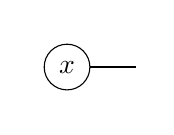
\begin{tikzpicture}[baseline=({N2.base}) ]
                \clip (-0.5,-0.5) rectangle (1,0.5);
                \node[circle, draw] (N2) at (0,0) {$x$};
                \node[] (N1) at (1,0) {};
                \draw  (N1) -- (N2) ;
            \end{tikzpicture}                                                     \\
            M                       & $M_{\alpha \beta}$      & 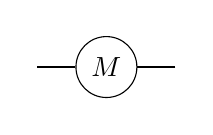
\begin{tikzpicture}[baseline={0cm-0.5*height("$=$")} ]
                \clip (-1,-0.5) rectangle (1,0.5);

                \node[circle, draw] (N2) at (0,0) {$M$};
                \node[] (N0) at (-1,0) {};
                \node[] (N1) at (1,0) {};

                \draw  (N1) -- (N2) ;
                \draw  (N0) -- (N2) ;

            \end{tikzpicture} \\

            $\Vec{x} \cdot \Vec{y}$ & $x_{\alpha} y_{\alpha}$ & 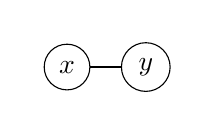
\begin{tikzpicture}[baseline=({N2.base}) ]
                \clip (-0.5,-0.5) rectangle (1.5,0.5);
                \node[circle, draw] (N2) at (0,0) {$x$};
                \node[circle, draw] (N1) at (1,0) {$y$};
                \draw  (N1) -- (N2) ;
            \end{tikzpicture} \\
        \end{tabular}
    \end{table}
\end{frame}

\begin{frame}{Tensor Networks: MPS}

    \begin{equation}
        C^{i_1 i_2 \cdots i_n} = Tr( C^{i_1} C^{i_2} \cdots C^{i_n} M )
    \end{equation}
    \begin{equation}
        \ctens  \; = \mpograph
    \end{equation}
\end{frame}

\begin{frame}{Tensor Networks: Operators}

    \begin{equation}
        \hat{O} =   \vcenter{\hbox{ \pepob{5}{3}{{
                            "-","-", "-","-",
                            "","","","",
                            "-","-", "-","-",}}{{
                            "-","-",
                            "","",
                            "","",
                            "","",
                            "-","-",}}{{
                            4,4,4,4,4,
                            13,0,0,0,13,
                            4,4,4,4,4,}} }}
    \end{equation}

    \begin{equation}
        \hat{O} \ket{\Psi} =  \vcenter{\hbox{ \pepob{5}{3}{{
                            "-","-", "-","-",
                            "","$\chi$","","",
                            "","$\chi$","","",}}{{
                            "-", "-",
                            "", "",
                            "", "",
                            "", "",
                            "-", "-",}}{{
                            4,4,4,4,4,
                            13,0,0,0,13,
                            13,0,0,0,13}}  }} =   \vcenter{\hbox{ \pepob{5}{2}{{
                            "-","-", "-","-",
                            "","$\chi^2$","",""}}{{
                            "-",
                            "",
                            "",
                            "",
                            "-"}}{{
                            4,4,4,4,4,
                            13,0,0,0,13}} }}
    \end{equation}

\end{frame}

\section{Linear Solver}

\begin{frame}{Linear Solver: Inversion Scheme}

    \begin{minipage}{0.4\textwidth}
        \only<1> { \begin{equation}
                \scalebox{0.9}{ \pepoat } \;  =  \; \scalebox{0.9}{\blockat}
            \end{equation}}
        \only<2-> {
            \begin{itemize}
                \only<2-> {\item Invert $A^i$ separately }
                      \only<2-3>{
                          \begin{itemize}
                              \item Fast
                              \item Numerically unstable
                          \end{itemize}
                      }
                      \only<4-> { \item Full inversion }
                      \only<4>{
                          \begin{itemize}
                              \item Slow
                              \item Stable for pseudoinverse
                          \end{itemize}
                      }
                      \only<5-> { \item Sparse full inversion }
                      \only<5>{
                          \begin{itemize}
                              \item $A^i = U^i \Sigma^i V^{i\dagger}$
                          \end{itemize}
                      }
            \end{itemize}
        }
    \end{minipage}
    \begin{minipage}{0.59\textwidth}
        \begin{equation}
            \only<1>  {  \vcenter{\hbox{   \scalebox{0.9}{  \pepoct }} } = \vcenter{\hbox{ \scalebox{0.9}{ \blockcta} }} }
            \only<2> { \vcenter{\hbox{  \scalebox{0.9}{  \pepocta } }}  =\vcenter{\hbox{ \scalebox{0.9}{  \blockcta }} }  }
            \only<3> { \vcenter{\hbox{ \scalebox{0.9}{  \pepoctb }}}  =\vcenter{\hbox{ \scalebox{0.9}{  \blockctb }} } }
            \only<4> { \vcenter{\hbox{ \scalebox{0.9}{  \pepoctc } }}  =\vcenter{\hbox{ \scalebox{0.9}{  \blockcta }} } }
            \only<5> { \vcenter{\hbox{\scalebox{0.9}{  \pepoctd }}}  =\vcenter{\hbox{ \scalebox{0.9}{  \blockcta }} } }
        \end{equation}
    \end{minipage}

    \only<2->{  \addtocounter{framenumber}{1} }

\end{frame}

\section{Construction}

\begin{frame}{Notation}
    \begin{equation}
        O^{0 0} = \mpo{1}{ {0,0}  }{ {"$i$",}  }{ {"$j$",}}{}{{"",}} = \mpob{1}{ {0,0}  }{ {"$i$",}  }{ {"$j$",}}{}{{"",}}
    \end{equation}

    \begin{equation}
        O^{0 1} O^{1 0} = \mpob{2}{ {0,1,0}  }{ {"$i_1$","$i_2$"}  }{ {"$j_1$","$j_1$",}}{}{{"",}}
    \end{equation}

\end{frame}

\begin{frame}{General idea}
    \begin{equation}
        \mpob{1}{ {0,0}  }{}{}{}{{"",}} = \exp \left( -\beta H(\mpob{1}{}{}{}{}{{"",}})   \right)
    \end{equation}

    \begin{equation}
        \begin{split}
            \mpob{2}{ {0,1,0}  }{}{}{}{{"",}}  = \exp -\beta H( & \mpob{2}{ {,,} }{}{}{}{{"",}}) \\
            - &\mpob{2}{ {0,0,0}  }{}{}{}{{"",}}
        \end{split}
    \end{equation}

\end{frame}

\begin{frame}{General idea}
    \begin{equation}
        \begin{split}
            \only<1> { \mpob{3}{ {0,1,1,0}  }{}{}{}{{,,,}}  = \exp -\beta H( &   \mpob{3}{ {,,,} }{}{}{}{{,,}})  \\
                - \; &\mpob{3}{ {0,0,0,0}  }{}{}{}{{,,,}}\\
                - \;&\mpob{3}{ {0,1,0,0}  }{}{}{}{{,,,}}\\
                - \; &\mpob{3}{ {0,0,1,0}  }{}{}{}{{,,,}}}
            \only<2> {  \mpob{3}{ {0,1,1,0}  }{}{}{}{{,,,}}    = \exp -\beta H( &   \mpob{3}{ {,,,} }{}{}{}{{,,}})  \\[10pt]
                - \; &\mpob{3}{ {,,,}  }{}{}{}{{,,,}}}
            \only<3> {  \boxed{ \mpob{3}{ {0,1,1,0}  }{}{}{}{{,,,}} } }
        \end{split}
    \end{equation}
\end{frame}

\subsection{1D}
\begin{frame}{1D: Variant A}
    \begin{subequations}
        \begin{align}
             & \mpob{1}{ {,}  }{}{}{}{{,,}}                                      \\
             & \mpob{2}{ {,"1",}  }{}{}{}{{,,}}                                  \\
             & \mpob{3}{ {,"1","1",}  }{}{}{}{{,,,}}                             \\
             & \mpob{4}{ {,"1","2","1",}  }{}{}{}{{,,,,,}}    \label{2sitepatch} \\
             & \mpob{5}{ {,"1","2","2","1",}  }{}{}{}{{,,,,,}} \; .
        \end{align}
    \end{subequations}
\end{frame}

\begin{frame}{1D: Variant E}
    \begin{subequations}
        \begin{align}
             & \mpob{1}{ {,}  }{}{}{}{{,,}}                          \\
             & \mpob{2}{ {,"1",}  }{}{}{}{{,,}}                      \\
             & \mpob{3}{ {,"1","1'",}  }{}{}{}{{,,,}}                \\
             & \mpob{4}{ {,"1","2","1'",}  }{}{}{}{{,,,,,}}          \\
             & \mpob{5}{ {,"1","2","2'","1'",}  }{}{}{}{{,,,,,}} \;.
        \end{align}
    \end{subequations}
\end{frame}

\begin{frame}{1D: Variant F}
    \begin{subequations}
        \begin{align}
             & \mpob{1}{ {,}  }{}{}{}{{,,}}                                         \\
             & \mpob{2}{ {,"1'",}  }{}{}{}{{,,}}+  \mpob{2}{ {,"1",}  }{}{}{}{{,,}} \\
             & \mpob{3}{ {,"1","1",}  }{}{}{}{{,,,}}                                \\
             & \mpob{4}{ {,"1","2","1",}  }{}{}{}{{,,,,,}} \; +  \nonumber          \\
             & \mpob{4}{ {,"1","2'","1",}  }{}{}{}{{,,,,,}}                         \\
             & \mpob{5}{ {,"1","2","2","1",}  }{}{}{}{{,,,,,}} \;.
        \end{align}
    \end{subequations}
\end{frame}

\subsection{2D}

\begin{frame}
    \begin{equation}
        O^{0000} =  \vcenter{ \hbox{ \pepob{4}{3}{{
                            "-","-","-",
                            "-","0","0",
                            "-","-","-"}}{{
                            "-","-",
                            "-","-",
                            "0","0",
                            "-","-"}}{{
                            1,1,4,1,
                            1,4,12,4,
                            1,1,4,1}} }} = \mpob{1}{ {,}  }{}{}{}{{,,}}
    \end{equation}
\end{frame}

\begin{frame}{2D: Linear Blocks}
    \begin{subequations}
        \begin{align}
             & \vcenter{\hbox{ \pepob{2}{2}{{"1",,}}{{,,}}{{0,0,1,1}} }}                                                                                                                                   \\[0.5cm]
             & \vcenter{\hbox{  \pepob{2}{2}{{"1","1",}}{{"1","1",}}{{0,0,0,1}} }}\;
            \vcenter{\hbox{  \pepob{3}{2}{{"1","1","1","1"}}{{"1","1","1","1"}}{{0,0,0,1,1,1}} }}                                                                                                          \\[0.5cm]
             & \vcenter{\hbox{  \pepob{3}{2}{{"1","1","1","1"}}{{"1","1","1","1"}}{{0,0,0,1,0,1}} \quad   \pepob{3}{3}{{"1","1","1","1","1","1",}}{{"1","1","1","1","1","1",}}{{1,0,1,0,0,0,1,0,1}}  }} \;
        \end{align}
    \end{subequations}
\end{frame}

\begin{frame}{2D: Nonlinear Blocks}
    \begin{equation}
        \vcenter{\hbox{   {\pepob{2}{2}{{"$\alpha$","$\alpha$",}}{{"$\alpha$","$\alpha$",}}{{0,0,0,0}}} }}
    \end{equation}

    \begin{equation}
        \vcenter{\hbox{     \pepob{5}{3}{{
                            "-","-", "-",     "-",
                            "-","1","$\beta$","-",
                            "-","-","$\alpha$","-"}}{{
                            "-","-",
                            "-","-",
                            "-","$\gamma$",
                            "-","$\alpha$",
                            "-","-"}}{{
                            1,1,1,1,1,
                            1,0,0,0,1,
                            1,1,0,0,1}} }} \; .
    \end{equation}
\end{frame}

\section{TFI Collapses}

\subsection{$g=0.0$}

\begin{frame}{TFI Phase Diagram: Classical Ising}
    \begin{minipage}{.75\textwidth}
        \begin{figure}
            \center
            \includegraphics[height=\textheight]{../Figuren/phasediag/g0/zoomed_small.pdf}
        \end{figure}
    \end{minipage}
    \begin{minipage}{.24\textwidth}
        \begin{table}[]
            \begin{tabular}{l|l }
                      & $T_c$    \\
                \hline           \\
                Fit   & 2.691(9) \\
                Exact & 2.691853 \\

            \end{tabular}
        \end{table}
    \end{minipage}
\end{frame}

\subsection{$g=2.9$}

\begin{frame}
    \begin{figure}
        \center
        \includegraphics[height=\textheight]{../Figuren/phasediag/g29/a.pdf}
    \end{figure}
\end{frame}

\section{Direct Results}

\begin{frame}{1D: Transverse Field Ising (TFI): full }

    \begin{figure}
        \center
        \includegraphics[height=\textheight]{../Figuren/benchmarking/t_ising.pdf}
    \end{figure}

\end{frame}

\begin{frame}{1D: Heisenberg XXX}

    \begin{figure}
        \center
        \includegraphics[height=\textheight]{../Figuren/benchmarking/t_heis_XXX.pdf}
    \end{figure}

\end{frame}

\subsection{2D Exact}

\begin{frame}{2D: Encodings + Error Measure}

    \begin{minipage}{.6\textwidth}
        \begin{itemize}
            \item Relative error $\epsilon$ more challenging
            \item Encodings based on A (order 5)
                  \begin{itemize}
                      \item \makebox[2.07cm]{No loops\hfill}$\vcenter{\hbox{\pepob{5}{3}{{
                                                    "-","-", "-",     "-",
                                                    "","","","",
                                                    "","-","",""}}{{
                                                    "-","",
                                                    "-","",
                                                    "-","",
                                                    "-","",
                                                    "-",""}}{{
                                                    1,1,1,1,1,
                                                    1,0,0,0,0,
                                                    1,1,0,1,1}} }} $
                      \item \makebox[2cm]{+Plaquette\hfill}$\vcenter{\hbox{{\pepob{2}{2}{{
                                                            "","",}}{{
                                                            "","",}}{{
                                                            0,0,
                                                            0,0}}} }}$
                      \item \makebox[2cm]{+Extensions\hfill}$\vcenter{\hbox{\pepob{5}{3}{{
                                                    "-","-", "-","-",
                                                    "","","","",
                                                    "","","",""}}{{
                                                    "-","",
                                                    "-","",
                                                    "-","",
                                                    "-","",
                                                    "-",""}}{{
                                                    1,1,1,1,1,
                                                    1,1,0,0,0,
                                                    1,1,0,0,1}} }} $
                  \end{itemize}
        \end{itemize}

    \end{minipage}
    \begin{minipage}{.39\textwidth}
        \begin{table}[]
            \begin{tabular}{l|l }
                           & $\chi$ \\
                \hline              \\
                no loops   & 21     \\
                plaquette  & 27     \\
                extensions & 43     \\
            \end{tabular}
        \end{table}

    \end{minipage}

\end{frame}

\begin{frame}{2D: Transverse Field Ising}

    \begin{figure}
        \center
        \includegraphics[height=\textheight]{../Figuren/benchmarking/2D_err_presentation}
    \end{figure}

\end{frame}

